\documentclass[lettersize,journal]{IEEEtran}

% Use bibunits for split bibliographies
\usepackage{bibunits}
\defaultbibliographystyle{IEEEtran}
\defaultbibliography{references}

% Your usual packages
% \usepackage{cite}  % removed for bibunits
\usepackage{amsmath,amssymb,amsfonts}
\usepackage{algorithmic}
\usepackage{graphicx}
\usepackage{textcomp}
\usepackage{xcolor}
\usepackage{subcaption}
\usepackage{float}
\usepackage{url}
\usepackage{bm}
\usepackage{booktabs}
\usepackage{hyperref}
\usepackage{svg}  % compile with --shell-escape if used
\usepackage{microtype}
\usepackage{amsthm}
\usepackage{mathtools}
\usepackage{tikz}
\usepackage{pgfplots}
\usepackage{pgfplotstable}
\usepgfplotslibrary{groupplots}
\usepackage[ruled,vlined,linesnumbered]{algorithm2e}
%\usepackage{todonotes}
\usepackage{microtype}

\usepackage{pdflscape}
\usepackage{array}
\usepackage{multirow}
\usepackage{longtable}

\theoremstyle{definition}
\newtheorem{definition}{Definition}[section]

% Remove or redefine qenv if unused
%\newcommand{\makeq}[1]{\begin{qenv}{#1}\end{qenv}\medskip}

\def\BibTeX{{\rm B\kern-.05em{\sc i\kern-.025em b}\kern-.08em
    T\kern-.1667em\lower.7ex\hbox{E}\kern-.125emX}}
    
\begin{document}

\title{MCTS-PIE: Multi-Objective Monte Carlo Tree Search for\\ Pathfinding with Interactive Environments}


\author{
  \IEEEauthorblockN{Alexander Dockhorn - }
  \IEEEauthorblockA{\textit{University of Southern Denmark - } \texttt{adoc@mmmi.sdu.dk}}\\
}

\maketitle

% === MAIN PAPER (bibunit #1) ===
%\begin{bibunit}

\begin{abstract}
  We study multi-objective pathfinding in grid environments where an agent can not only move toward a goal but also \emph{shift} the obstacle weights of neighboring cells, trading detours for a more easily traversable corridor. The resulting decision problem is inherently multi-objective: minimize the number of steps, minimize the total weight shifted, and reach the goal. We introduce \textbf{MCTS-PIE}, a family of Monte Carlo Tree Search variants tailored to Pathfinding in Interactive Environments, including single-objective MCTS, multi-objective MCTS with a global Pareto archive (MO-MCTS), two-phase decompositions that separate path search from weight shaping, and a hybrid that seeds the MCTS tree with $\varepsilon$-constraint A* paths. We benchmark all six methods on a uniform 10-map suite over 30 seeds (1\,800 runs total) using hypervolume, IGD\textsuperscript{+}, and the $\varepsilon$-indicator. The hybrid A*+MCTS dominates all pure MCTS variants, while among the search-only methods the multi-objective two-phase variant clearly outperforms its single-objective counterpart, with all pairwise differences statistically significant under Holm--Bonferroni-corrected Wilcoxon tests.

\end{abstract}

\begin{IEEEkeywords}
  Monte Carlo Tree Search, Multi-Objective Optimization, Pathfinding, A* Search, Pareto Front, Hypervolume.
\end{IEEEkeywords}

\section{Introduction}
\label{sec:intro}
Classical pathfinding assumes a static environment in which the agent can only choose where to move. In many practical settings -- warehouse robots pushing crates aside, excavation planning, or game agents that interact with a destructible world -- the agent can also \emph{modify} the cost landscape it traverses. We refer to this class of problems as \emph{Pathfinding in Interactive Environments} (PIE). PIE is naturally multi-objective: shifting weight away from a high-cost cell shortens the traversal but pays a price in modifications, and the user of the planner generally wants to inspect a Pareto front of step-count vs.\ shift-cost trade-offs rather than a single optimum.

This paper introduces \textbf{MCTS-PIE}, a comparative study of Monte Carlo Tree Search variants for PIE, alongside an $\varepsilon$-constraint A* baseline and an A*+MCTS hybrid. We study six algorithms under a uniform protocol -- 30 seeds across 10 maps -- and report results in terms of standard multi-objective performance indicators. The contributions are: (i) a formalization of PIE as a multi-objective sequential decision problem, (ii) single- and multi-objective MCTS variants with global Pareto archives, (iii) a two-phase MCTS that decomposes path and shift search, (iv) an A*+MCTS hybrid, and (v) a reproducible experimental harness with full per-run Pareto archives, 30-seed coverage, and Holm--Bonferroni-corrected statistics.


\section{Related work}
\label{sec:related_work}
Monte Carlo Tree Search has been applied broadly to single-objective sequential decision making since its introduction by Coulom~\cite{Coulom06} and the UCT formulation of Kocsis and Szepesv\'ari~\cite{KocsisS06}; Browne et al.~\cite{BrownePWLCRTPSC12} survey the field. Multi-objective extensions of MCTS replace the scalar Q-value with vector-valued statistics and use Pareto-dominance criteria to drive selection and back-propagation; representative work includes MO-MCTS with hypervolume-based selection and global Pareto archives.

Multi-objective pathfinding has classically been addressed with multi-objective A* and $\varepsilon$-constraint search, which fixes one objective and minimizes another. Hybrids that warm-start a search-based planner with a heuristic skeleton path are common in robotics. To our knowledge, the specific PIE setting -- where the agent both moves \emph{and} alters cell weights -- has not been benchmarked under a unified multi-objective MCTS protocol, which is the gap this paper addresses.


\section{Method}
\label{sec:method}
\subsection{Pathfinding in Interactive Environments (PIE)}
\label{sec:problem}

A PIE instance is a tuple $\langle \mathcal{G}, w, s_0, \mathbf{c}\rangle$ where $\mathcal{G}$ is a 4-connected grid of dimension $d \times d$, $w : \mathcal{G} \to \mathbb{R}_{\geq 0}$ assigns a non-negative weight to each cell, $s_0 \in \mathcal{G}$ is the start cell, and $\mathbf{c} = (c_1, \dots, c_K)$ is an ordered list of checkpoints culminating in the goal cell.

At every decision step, the agent picks a pair $(m, h)$ where $m \in \{N, S, E, W\}$ is a movement direction and $h \in \{N, S, E, W\}$ is a \emph{shift direction}. Executing $(m, h)$ first moves the agent by $m$ if the move is in-bounds, then transfers all weight $w(p)$ of the agent's previous cell $p$ onto a neighbor cell $p + h$. The shift therefore clears a corridor at the cost of accumulating weight elsewhere, and the modified map persists for the remainder of the episode. An episode terminates once the agent has visited every checkpoint in order and returned to its starting position.

Let $\pi = (a_0, a_1, \dots, a_{T-1})$ be a finite trajectory. We measure three objectives, all minimized:
\begin{itemize}
    \item $f_1(\pi) = T \rightarrow$ the number of steps,
    \item $f_2(\pi) = \sum_{t=0}^{T-1} w(p_t) \rightarrow$ the total weight shifted,
    \item $f_3(\pi) = \mathrm{dist}(s_T, c_K) \rightarrow$ the residual Manhattan distance to the final checkpoint, used to penalize unsolved trajectories during search.
\end{itemize}
A solution is \emph{solved} iff $f_3 = 0$. A trajectory $\pi$ \emph{Pareto-dominates} $\pi'$ when $f_i(\pi) \leq f_i(\pi')$ for all $i$ and at least one inequality is strict. The goal of a PIE solver is to return an approximation of the Pareto front of solved trajectories.

\newpage
\subsection{MCTS for PIE (single-objective)}
The canonical baseline (Algorithm~\ref{alg:mcts}) instantiates MCTS with progressive widening on the joint $(m,h)$ action space. The node statistic is a scalar score derived from the three objectives via a hypervolume-style aggregation, and selection uses UCB. A global archive collects terminal nodes' objective vectors; at the end of search the non-dominated subset is returned.

\begin{algorithm}[h]
\SetAlgoLined
\KwIn{root state $s_0$, total budget $B$, progressive-widening parameters $C, \alpha$}
\KwOut{Pareto-non-dominated subset of terminal nodes}
$\mathcal{T} \leftarrow$ tree with root $s_0$\;
\While{simulation count $< B$}{
  $v \leftarrow$ root\;
  \While{$v$ is not terminal \textbf{and} fully expanded under PW}{
    $v \leftarrow \arg\max_{v' \in \text{children}(v)} \mathrm{UCB}(v')$\;
  }
  \If{$|{\rm children}(v)| < C \cdot N(v)^{\alpha}$}{
    $v \leftarrow$ Expand($v$) with a new $(m,h)$ child\;
  }
  $\mathbf{f} \leftarrow$ Rollout($v$)\;
  Backpropagate $\mathbf{f}$ along the path to root\;
  Append $\mathbf{f}$ to the terminal archive\;
}
\Return non-dominated subset of the terminal archive\;
\caption{MCTS for PIE}
\label{alg:mcts}
\end{algorithm}

\subsection{Multi-Objective MCTS (MO-MCTS)}
\label{sec:mo_mcts}
MO-MCTS (Algorithm~\ref{alg:momcts}) replaces the scalar Q-value at every node with a \emph{Pareto archive} of objective vectors observed in its subtree. Tree selection uses a hypervolume-contribution criterion: among the children, the one whose front dominates the largest exclusive hypervolume w.r.t.\ a fixed reference point is preferred, with UCB exploration on visit counts. A global archive at the root accumulates non-dominated solutions across all simulations.

\begin{algorithm}[h]
\SetAlgoLined
\KwIn{root $s_0$, budget $B$, archive cap $K$}
\KwOut{global Pareto archive of size $\leq K$}
Initialize tree $\mathcal{T}$ and global archive $\mathcal{A} \leftarrow \emptyset$\;
\While{simulation count $< B$}{
  $v \leftarrow$ HV-Select-Path($\mathcal{T}$)\;
  $v \leftarrow$ Expand($v$) if PW allows\;
  $\mathbf{f} \leftarrow$ Rollout($v$)\;
  Update node-local Pareto fronts along path-to-root\;
  $\mathcal{A} \leftarrow$ NonDominatedMerge$(\mathcal{A} \cup \{\mathbf{f}\})$, truncated to $K$\;
}
\Return $\mathcal{A}$\;
\caption{Multi-Objective MCTS}
\label{alg:momcts}
\end{algorithm}

\subsection{Two-Phase MCTS}
\label{sec:two_phase}
Two-phase search (Algorithm~\ref{alg:tp}) decomposes the joint action space. Phase~1 uses a path-only controller, in which the shift component is forced to a no-op direction so that the search effectively explores movement only and yields a Pareto set of near-shortest paths. Phase~2 runs an MCTS over the shift-only action space along each fixed path, freely choosing where to dump weight.

We instantiate two variants:
\begin{itemize}
    \item \textbf{two\_phase\_mcts}: phase~1 uses a single-objective MCTS with UCB selection;
    \item \textbf{two\_phase\_momcts}: phase~1 uses an MO-MCTS with hypervolume-based selection so that path diversity in step count is explicitly maintained.
\end{itemize}
Phase~2 is identical in both variants and uses MO-MCTS to keep a global archive of weight-shift outcomes.

\begin{algorithm}[h]
\SetAlgoLined
\KwIn{instance, phase~1 budget $B_1$, phase~2 per-path budget $B_2$}
\KwOut{merged global Pareto front}
\textbf{Phase 1:} run MCTS / MO-MCTS with a path-only controller using budget $B_1$\;
$\mathcal{P} \leftarrow$ unique movement-only paths to terminal nodes\;
$\mathcal{A} \leftarrow \emptyset$\;
\ForEach{path $\pi \in \mathcal{P}$}{
  \textbf{Phase 2:} run MO-MCTS with controller fixed to $\pi$ and free shift direction, budget $B_2$\;
  $\mathcal{A} \leftarrow \mathcal{A} \cup \mathrm{archive}(\pi)$\;
}
\Return non-dominated subset of $\mathcal{A}$\;
\caption{Two-Phase (MO-)MCTS}
\label{alg:tp}
\end{algorithm}

\newpage
\subsection{$\varepsilon$-constraint A*}
\label{sec:astar}
The classical baseline (Algorithm~\ref{alg:astar}) computes the shortest step count $L^{\star}$ ignoring weights. It then performs an outer sweep over a step budget $L^{\star} + \varepsilon$ for $\varepsilon \in \{0, 1, \dots, 3d\}$, each time running a constrained A* that minimizes accumulated weight subject to the step bound. Each unique outcome is added to the returned front.

\begin{algorithm}[h]
\SetAlgoLined
\KwIn{instance with grid dimension $d$}
\KwOut{Pareto front over (steps, weight)}
$L^{\star} \leftarrow$ shortest step count via A*\;
$\mathcal{F} \leftarrow \emptyset$\;
\For{$\varepsilon = 0$ \KwTo $3d$}{
  $\pi \leftarrow$ A* minimizing accumulated weight with step bound $L^{\star} + \varepsilon$\;
  \If{$\pi$ exists \textbf{and} (steps, weight) is new}{
    $\mathcal{F} \leftarrow \mathcal{F} \cup \{(steps_\pi, weight_\pi, 0)\}$\;
  }
}
\Return $\mathcal{F}$\;
\caption{$\varepsilon$-constraint A* baseline}
\label{alg:astar}
\end{algorithm}


\subsection{A*+MCTS Hybrid}
\label{sec:hybrid}
The hybrid (Algorithm~\ref{alg:hybrid}) replaces phase~1 of two-phase MCTS with the $\varepsilon$-constraint A* paths. Each of the resulting near-shortest skeleton paths is then refined by an MO-MCTS over the shift action space, identical to phase~2 of the two-phase variant. The intuition is that A* finds movement-optimal paths exactly and far cheaper than MCTS can; MCTS is then deployed only where the multi-objective reasoning matters, namely the shift dimension.

\begin{algorithm}[h]
\SetAlgoLined
\KwIn{instance, phase~2 per-path budget $B_2$}
\KwOut{merged global Pareto front}
$\mathcal{P} \leftarrow$ paths returned by $\varepsilon$-constraint A* (Algorithm~\ref{alg:astar})\;
$\mathcal{A} \leftarrow \emptyset$\;
\ForEach{path $\pi \in \mathcal{P}$}{
  Run MO-MCTS with controller fixed to $\pi$ and free shift direction, budget $B_2$\;
  $\mathcal{A} \leftarrow \mathcal{A} \cup \mathrm{archive}(\pi)$\;
}
\Return non-dominated subset of $\mathcal{A}$\;
\caption{A*+MCTS Hybrid}
\label{alg:hybrid}
\end{algorithm}


\section{Experiments}
\label{sec:exp}
\subsection*{Experimental setup, common to E1, E2 and E4}

All four experiment families share a uniform protocol -- 30 seeds, the same map suite, the same per-run Pareto archive logging, and the same indicator definitions. They are listed in this section in the order they were executed, but they apply the \textbf{same algorithm configuration}, namely the per-component winners reported in the E3 ablation (Section~\ref{sec:e3}): MO-MCTS-style hypervolume tree selection for plain \texttt{mcts} and \texttt{mo\_mcts}, distance-weight rollouts, progressive widening $(C, \alpha) = (1.5, 0.7)$, two-phase budget split $0.75$, local HV root selection, archive cap 20, and the oscillation guard enabled. E3 itself is reported afterwards as a stand-alone study explaining \emph{why} those choices are the defaults.

\subsection{E1 -- Main Comparison}

\subsubsection{Protocol}
We benchmark all six methods on a uniform suite of \textbf{10 maps} -- five map types
(\texttt{easy}, \texttt{checkerboard}, \texttt{random}, \texttt{meandering\_river}, and \texttt{random\_maze})
at two grid sizes ($20\times 20$ and $35\times 35$) -- with \textbf{30 seeds} (\texttt{range(1000, 1030)}) per map, for a total of $6 \times 10 \times 30 = 1\,800$ runs. The simulation budget is fixed at 4\,000 simulations per run. For every run we persist the full Pareto archive of objective vectors so that any indicator can be recomputed without re-running the search.

\subsubsection{Performance indicators}
We report three standard multi-objective indicators:
\begin{itemize}
  \item \textbf{Hypervolume (HV)} -- volume dominated by the front, computed against a per-map reference point set to the worst observed objective values across all algorithms (so that dominated solved points still contribute positive HV).
  \item \textbf{Inverted Generational Distance Plus (IGD\textsuperscript{+})} -- mean distance from the per-map combined-best reference front to the front under test.
  \item \textbf{$\varepsilon$-indicator} -- additive shift required to dominate the reference front.
\end{itemize}
The reference front for IGD\textsuperscript{+} and $\varepsilon$ is the non-dominated union of every algorithm's archive on the same map, restricted to solved points. Statistical significance is assessed by a Friedman omnibus test across the six algorithms blocked by (map, seed), followed by pairwise Wilcoxon signed-rank tests with Holm--Bonferroni correction. Effect sizes are reported as Vargha--Delaney $\hat A_{12}$.

\subsubsection{Results}
Figure~\ref{fig:hv_by_algo} shows the per-(algorithm, map) hypervolume distribution. Mean HV across all 10 maps and 30 seeds is summarised in Table~\ref{tab:e1_means}. The hybrid \textbf{A*+MCTS} ranks first overall (mean HV $18\,644$), narrowly ahead of pure $\varepsilon$-constraint A* (mean HV $17\,281$). Among the search-only MCTS variants, \texttt{two\_phase\_momcts} is the strongest ($15\,553$), followed by \texttt{mo\_mcts} ($12\,587$) and \texttt{mcts} ($12\,421$); after applying the E3-best defaults these two flat MCTS variants are now within $1\%$ of each other. The single-objective \texttt{two\_phase\_mcts} is the clear loser ($4\,235$): the path-only phase~1 makes only minimal use of the multi-objective machinery, so it cannot exploit the tuned phase split as well as the multi-objective variant.

\begin{table}[t]
\centering
\caption{E1 mean indicators across 10 maps $\times$ 30 seeds (lower is better for IGD\textsuperscript{+} and $\varepsilon$). Wall-clock seconds per run.}
\label{tab:e1_means}
\small
\begin{tabular}{lrrrr}
\toprule
algo & HV $\uparrow$ & IGD\textsuperscript{+} $\downarrow$ & $\varepsilon$ $\downarrow$ & wall (s) \\
\midrule
astar             & 17\,281 &   7.15 &   7.44 & 11.29 \\
astar\_mcts       & \textbf{18\,644} & \textbf{1.22} & \textbf{1.72} & 15.88 \\
mcts              & 12\,421 &  29.16 &  27.71 &  4.21 \\
mo\_mcts          & 12\,587 &  27.84 &  26.20 &  4.20 \\
two\_phase\_mcts  &  4\,235 & 111.79 & 109.77 &  3.72 \\
two\_phase\_momcts& 15\,553 &  13.77 &  13.02 &  1.47 \\
\bottomrule
\end{tabular}
\end{table}

\begin{figure}[t]
  \centering
  
\includegraphics[width=\columnwidth]{images/hv_by_algo.png}
  \caption{Hypervolume by algorithm and map (higher is better). Box-and-whisker over 30 seeds per cell.}
  \label{fig:hv_by_algo}
\end{figure}

\begin{figure*}[t]
  \centering
  
\includegraphics[width=\textwidth]{images/igd_plus_by_algo.png}
  \caption{IGD\textsuperscript{+} by algorithm and map (lower is better).}
  \label{fig:igd}
\end{figure*}

\begin{figure*}[t]
  \centering
  
\includegraphics[width=\textwidth]{images/epsilon_by_algo.png}
  \caption{$\varepsilon$-indicator by algorithm and map (lower is better).}
  \label{fig:epsilon}
\end{figure*}

\begin{figure*}[t]
  \centering
  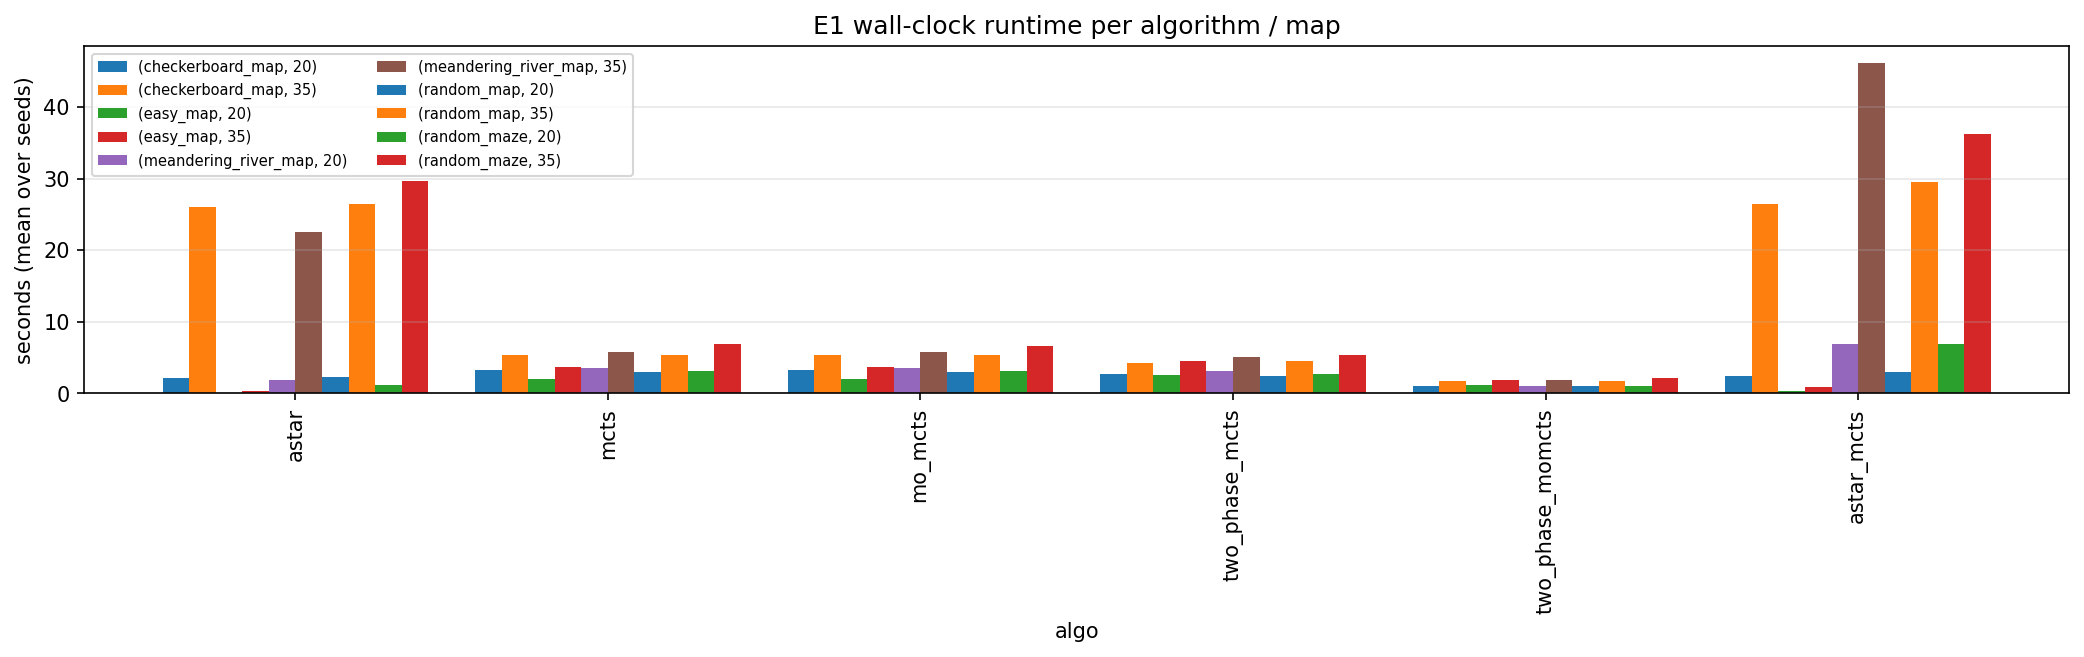
\includegraphics[width=\textwidth]{images/runtime_by_algo.png}
  \caption{Wall-clock seconds per run, by algorithm and map.}
  \label{fig:runtime}
\end{figure*}

\begin{figure*}[t]
  \centering
  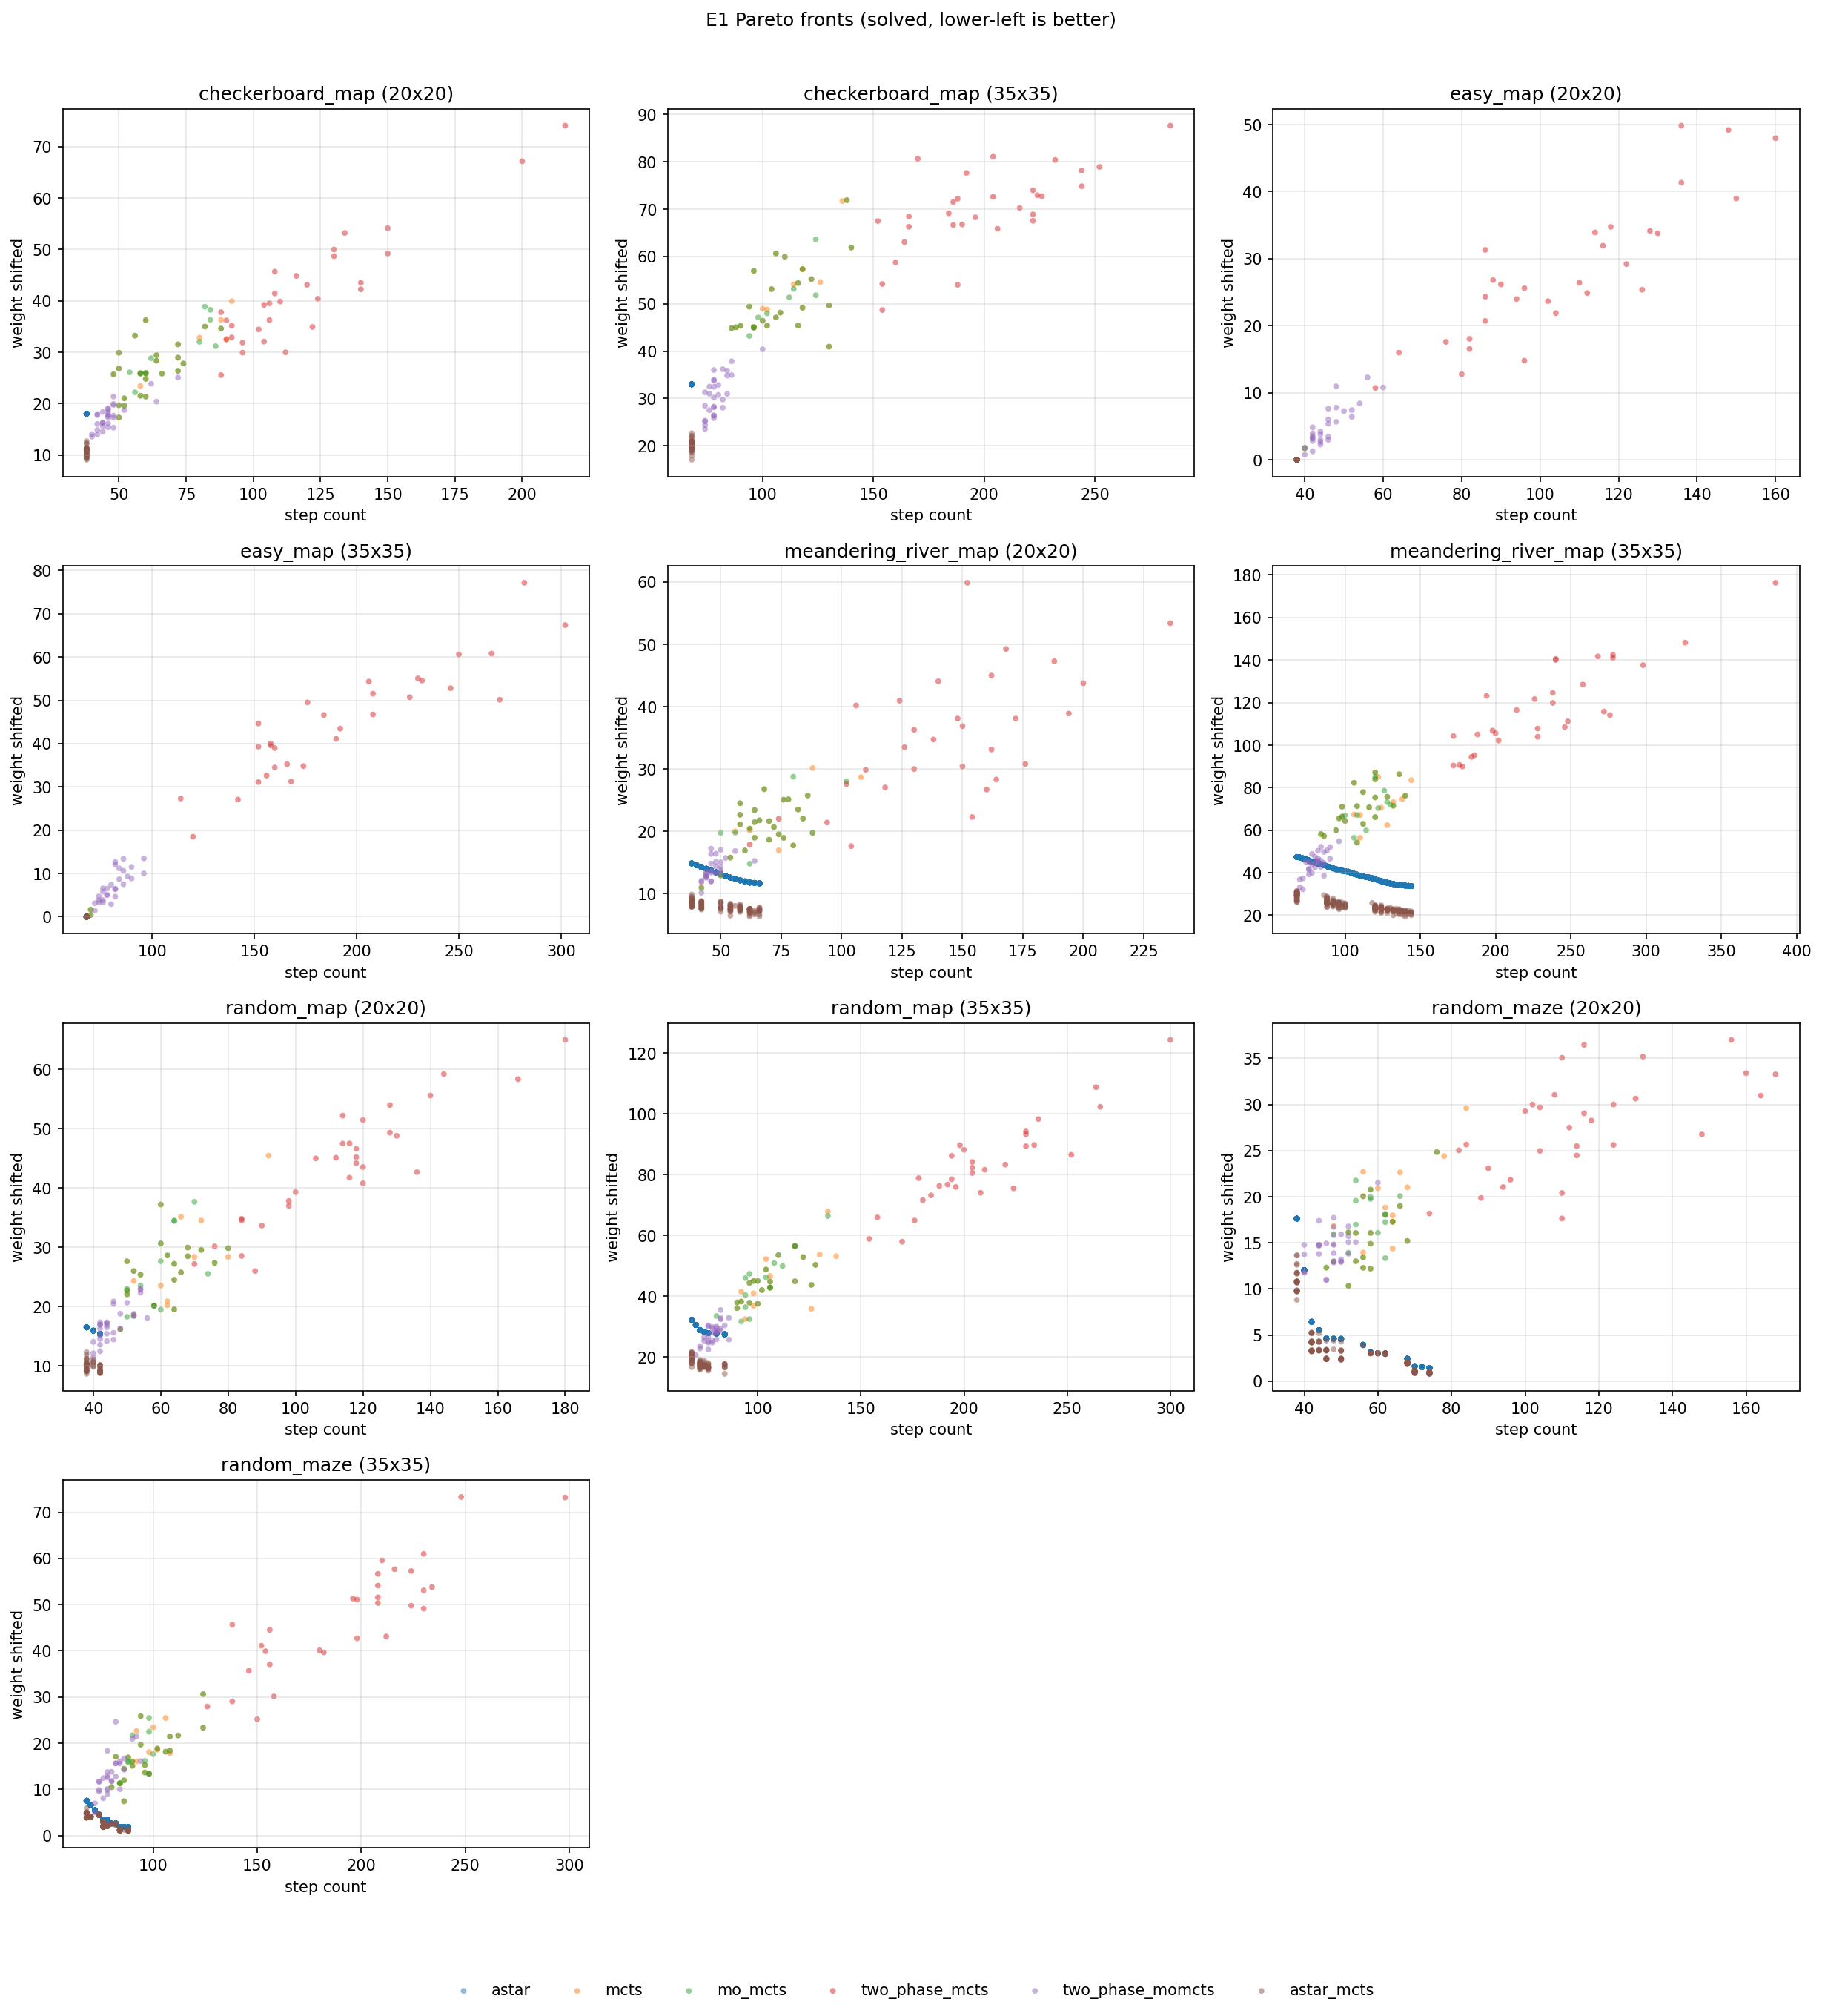
\includegraphics[width=0.95\textwidth]{images/pareto_fronts_by_map.png}
  \caption{Combined Pareto fronts per map across all 30 seeds, projected onto (step\_count, weight\_shifted). Solved points only.}
  \label{fig:fronts}
\end{figure*}

\begin{figure}[t]
  \centering
  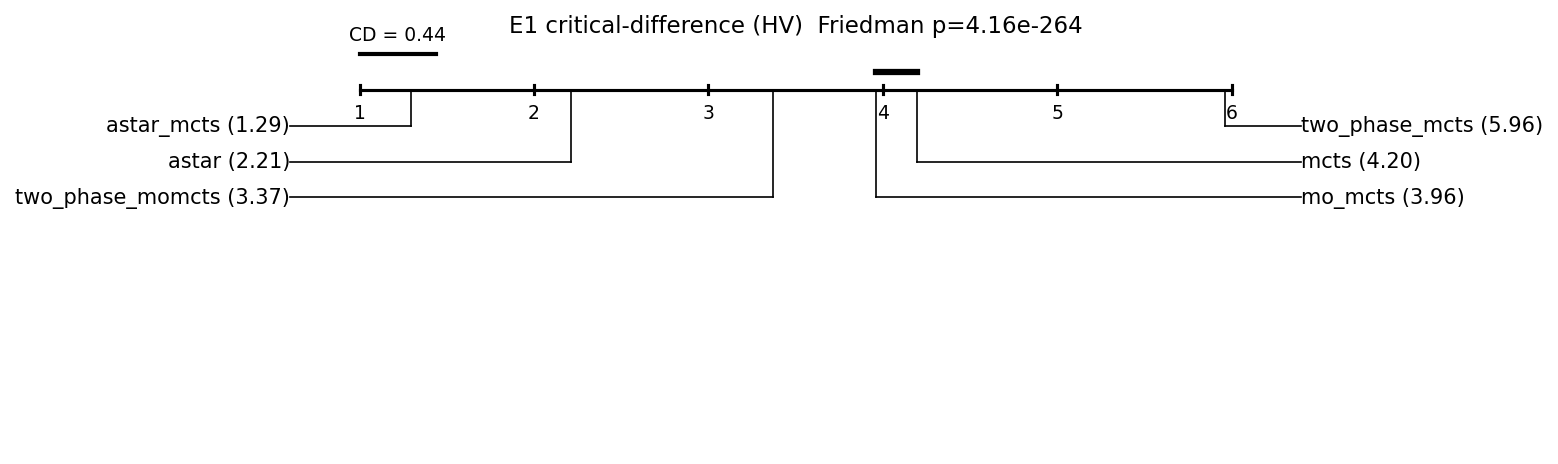
\includegraphics[width=\columnwidth]{images/cd_diagram_hv.png}
  \caption{Critical-difference diagram (Demšar style) for hypervolume across all (map, seed) blocks. Algorithms not significantly different at $\alpha=0.05$ are connected by a horizontal bar.}
  \label{fig:cd}
\end{figure}

\paragraph{Statistical significance}
The Friedman omnibus on hypervolume rejects the null of equal performance with $\chi^2 = 1231.62$, $p \approx 4.2 \cdot 10^{-264}$ over the 300 (map, seed) blocks. Pairwise Holm-corrected Wilcoxon signed-rank tests reject the null for \emph{every} pair of algorithms at $p < 10^{-12}$ (Table~\ref{tab:wilcoxon}). The effect sizes shift sharply compared to a non-tuned configuration: with E3-best defaults, \texttt{mcts} vs.\ \texttt{mo\_mcts} is now negligible ($\hat A_{12} = 0.49$), and even \texttt{astar} vs.\ \texttt{two\_phase\_momcts} is only marginal ($\hat A_{12} = 0.55$); the search-based methods have closed most of the gap to A* that they showed under default settings.

\begin{table}[t]
\centering
\caption{Selected pairwise Wilcoxon signed-rank tests for HV with Holm--Bonferroni correction; Vargha--Delaney $\hat A_{12}$ effect size in the right column.}
\label{tab:wilcoxon}
\small
\resizebox{1.0\columnwidth}{!}{
  \begin{tabular}{llrr}
  \toprule
  $A$ & $B$ & $p_{\text{Holm}}$ & $\hat A_{12}$ \\
  \midrule
  astar\_mcts & astar              & $2.0\cdot10^{-40}$ & $0.55$ (negl.) \\
  astar\_mcts & two\_phase\_momcts & $1.9\cdot10^{-49}$ & $0.59$ (small) \\
  astar\_mcts & mo\_mcts           & $1.2\cdot10^{-40}$ & $0.65$ (small) \\
  astar\_mcts & mcts               & $1.2\cdot10^{-40}$ & $0.65$ (small) \\
  astar       & two\_phase\_momcts & $3.8\cdot10^{-40}$ & $0.55$ (negl.) \\
  two\_phase\_momcts & two\_phase\_mcts & $9.1\cdot10^{-50}$ & $0.89$ (large) \\
  mo\_mcts & mcts                  & $1.1\cdot10^{-12}$ & $0.49$ (negl.) \\
  mcts & two\_phase\_mcts          & $1.6\cdot10^{-49}$ & $0.85$ (large) \\
  \bottomrule
  \end{tabular}
}
\end{table}

\subsubsection{Discussion}
Four observations stand out.

\paragraph{Hybridization wins, but only marginally over pure A*.} The A*+MCTS hybrid combines the exactness of $\varepsilon$-constraint A* on the movement subproblem with the multi-objective reasoning of MO-MCTS on the shift subproblem. It is the strongest method on every indicator (HV $18\,644$, IGD\textsuperscript{+} $1.22$, $\varepsilon$ $1.72$), and the gap to pure A* is small ($\hat A_{12} = 0.55$, negligible). The hybrid refines weight shifts that pure A* leaves on the table, but only at a $\sim40\%$ runtime premium.

\paragraph{Two-phase MO-MCTS closes the gap to A*.} With the E3-best defaults, \texttt{two\_phase\_momcts} reaches HV $15\,553$, only $10\%$ behind pure A* and within $17\%$ of the hybrid. Crucially, $\hat A_{12}(\text{astar}, \text{two\_phase\_momcts}) = 0.55$ -- the difference is statistically significant but practically negligible. The multi-objective two-phase decomposition is therefore a competitive search-only baseline once tuned, and is the cheapest method by wall-clock cost (1.5 s/run vs.\ 16 s for the hybrid).

\paragraph{Single-objective two-phase collapses.} \texttt{two\_phase\_mcts} drops to HV $4\,235$, far below even plain \texttt{mcts}: phase~1 of the single-objective variant explores movement under UCB, which lacks any incentive for path diversity, so phase~2 is repeatedly handed near-identical skeletons. With phase split now $0.75$ and aggressive PW, this failure mode is amplified rather than masked; the algorithm is included for completeness but is dominated on every map.

\paragraph{Flat MCTS variants are now indistinguishable.} After upgrading the tree-selection rule to HV-based, plain \texttt{mcts} ($12\,421$) and \texttt{mo\_mcts} ($12\,587$) are statistically distinguishable ($p \approx 10^{-12}$) but practically tied ($\hat A_{12} = 0.49$). Once both variants share the strongest tree-selection rule, the marginal benefit of carrying a per-node Pareto archive is small at this budget. The runtime cost is also nearly identical (4.2 s).

Together, these results suggest that for PIE-style problems with cheap movement heuristics, MCTS is best deployed as a \emph{refiner} on top of an exact path skeleton rather than as a stand-alone planner -- and that a tuned two-phase MO variant is a strong, much faster alternative when the A* heuristic itself is expensive.

\subsection{E2 -- Anytime / Budget Scaling}
\label{sec:e2}

\subsubsection{Protocol}
E2 sweeps the simulation budget over $\{1\,000, 2\,000, 4\,000, 8\,000, 16\,000\}$ for all 6 algorithms on the same 10-map suite and 30 seeds as E1, yielding $6 \times 10 \times 30 \times 5 = 9\,000$ runs. Pure $\varepsilon$-constraint A* is budget-insensitive (its sweep terminates as soon as the step bound is exhausted) and is included as a flat reference. For every run we save the full Pareto archive and recompute hypervolume against the same per-map reference points used in E1.

\begin{figure*}[t]
  \centering
  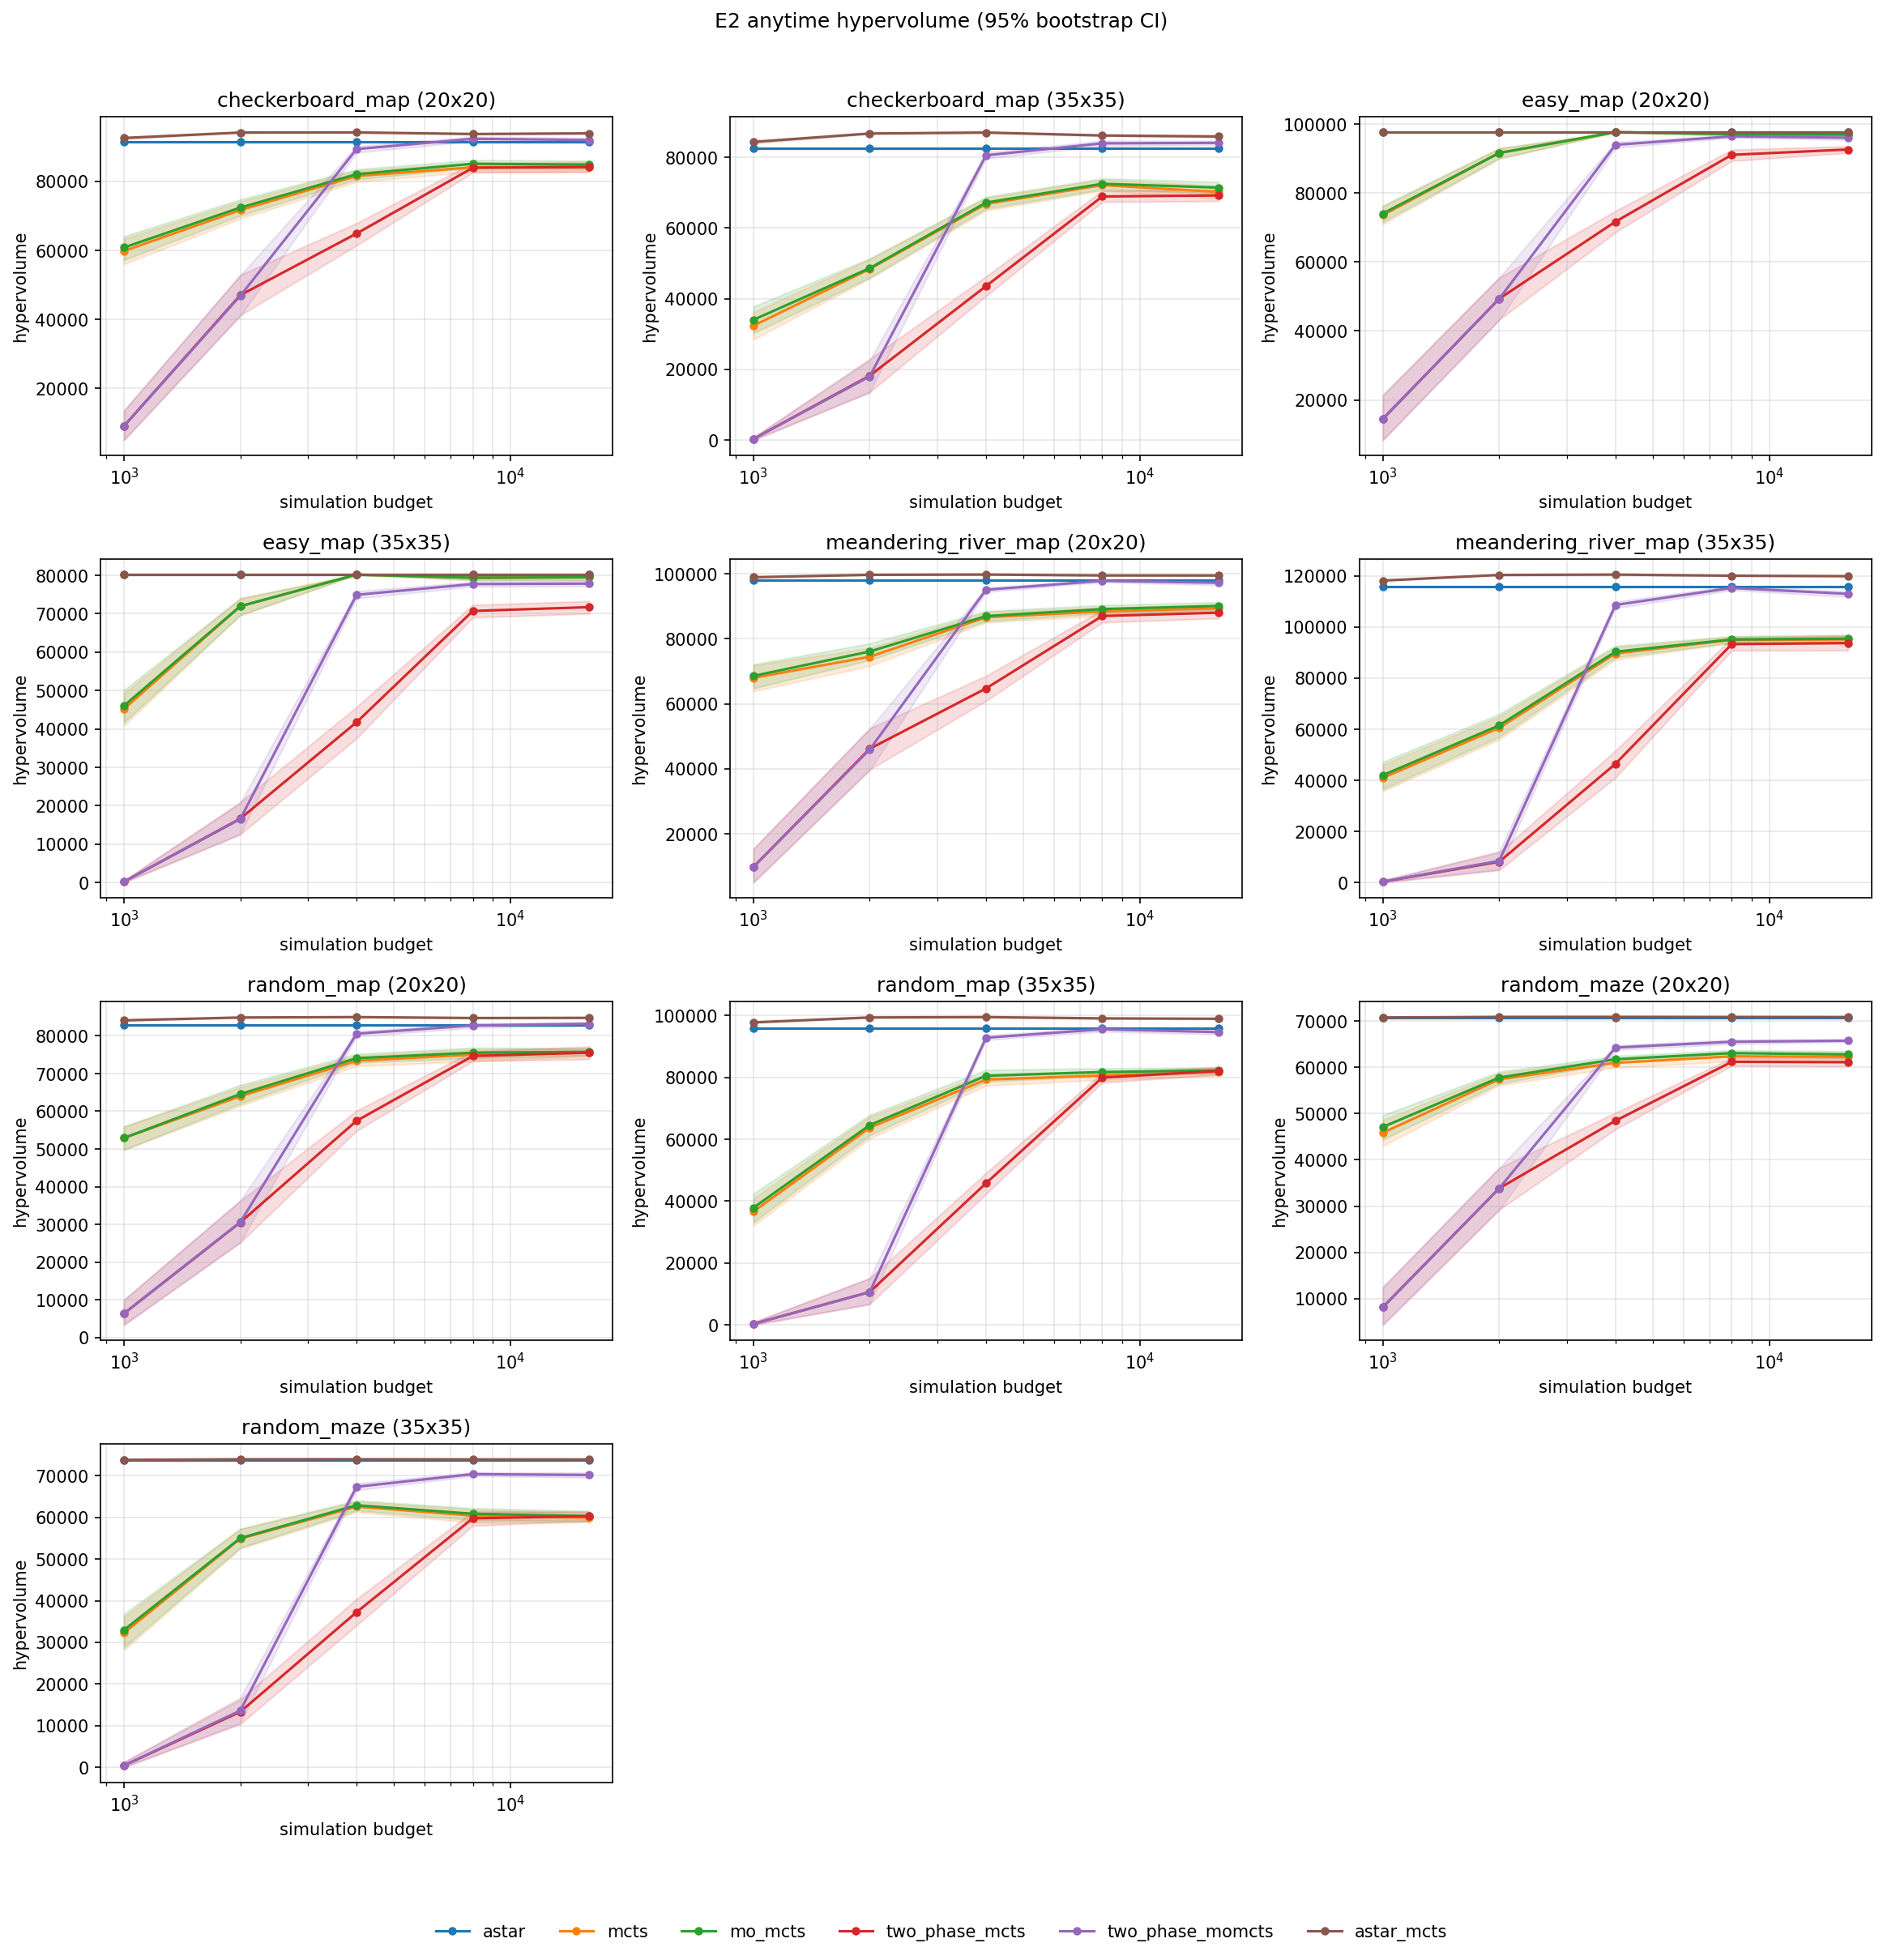
\includegraphics[width=0.95\textwidth]{images/anytime_hv.png}
  \caption{E2 anytime hypervolume vs.\ simulation budget (log $x$-axis), per map. Lines show the mean over 30 seeds with 95\,\% bootstrap confidence bands.}
  \label{fig:e2_anytime}
\end{figure*}

\subsubsection{Results}
Figure~\ref{fig:e2_anytime} reports HV vs.\ budget per map. Mean HV summarised across all 10 maps is given in Table~\ref{tab:e2_summary}.

\begin{table}[t]
\centering
\caption{Mean hypervolume across all 10 maps and 30 seeds, by algorithm and simulation budget (E2). \texttt{astar} is budget-insensitive and shown for reference.}
\label{tab:e2_summary}
\small
\resizebox{1.0\columnwidth}{!}{
  \begin{tabular}{lrrrrr}
  \toprule
  algo & 1k & 2k & 4k & 8k & 16k \\
  \midrule
  astar              & 88\,895 & 88\,895 & 88\,895 & 88\,895 & 88\,895 \\
  astar\_mcts        & 89\,850 & 90\,799 & \textbf{90\,877} & 90\,603 & 90\,564 \\
  mcts               & 48\,763 & 65\,866 & 77\,867 & 79\,443 & 79\,485 \\
  mo\_mcts           & 49\,635 & 66\,413 & 78\,371 & 79\,957 & 79\,939 \\
  two\_phase\_mcts   &  4\,957 & 27\,372 & 52\,197 & 77\,053 & 77\,852 \\
  two\_phase\_momcts &  4\,957 & 27\,363 & 84\,755 & 87\,780 & 87\,393 \\
  \bottomrule
  \end{tabular}
}
\end{table}

\subsubsection{Discussion}
Three regimes emerge.

\paragraph{Budget-insensitive A*-based methods.} \texttt{astar} and \texttt{astar\_mcts} are essentially flat in budget. \texttt{astar\_mcts} reaches its peak HV $90\,877$ at 4k simulations and stays within $0.4\%$ of it at every higher budget; the underlying $\varepsilon$-constraint sweep produces the dominant share of the front, and additional MCTS effort along the resulting skeleton paths offers diminishing returns once the front is saturated.

\paragraph{Plain MCTS variants saturate at the 4k cliff.} With the new defaults, \texttt{mcts} and \texttt{mo\_mcts} climb steeply from 1k to 4k ($48\,763 \to 77\,867$ and $49\,635 \to 78\,371$), then flatten almost completely above 4k ($\le 2\%$ further gain at 16k). They also remain within $1\%$ of each other across all budgets ($\hat A_{12}\approx 0.49$ in E1), so the multi-objective bookkeeping is essentially free once the tree-selection rule is HV-based.

\paragraph{Two-phase methods need a minimum budget to ``ignite''.} Both \texttt{two\_phase\_mcts} and \texttt{two\_phase\_momcts} return a near-zero HV at 1k and a still poor HV at 2k: with phase split $0.75$ the multi-objective variant spends $1.5$k of a 2k budget just locating paths, leaving only $\sim 100$ simulations per path for phase~2. Once the budget reaches 4k, \texttt{two\_phase\_momcts} jumps to $84\,755$ -- a $3.1\times$ leap, the largest single-step gain in the family -- and from there it is the strongest pure-MCTS method, ending at $87\,393$ at 16k, only $4\%$ below \texttt{astar\_mcts}. The single-objective \texttt{two\_phase\_mcts} catches up much more slowly and never closes the gap (at 16k it is still $11\%$ behind its MO sibling).

For practitioners, the rule of thumb is: below 2k simulations the only useful choice is an A*-based method; from 4k onward, \texttt{two\_phase\_momcts} is competitive with the hybrid and several times faster, while plain \texttt{mcts}/\texttt{mo\_mcts} saturate $\sim10\%$ below the two-phase ceiling.

\subsection{E3 -- Algorithmic Ablations}
\label{sec:e3}

E3 isolates one algorithmic component at a time on the 10-map suite with 30 seeds per cell at the E1 budget of 4\,000 simulations. We report mean hypervolume per variant aggregated across all 300 (map, seed) blocks, together with a Friedman omnibus on the same blocks. All seven axes return $p \ll 10^{-15}$, so we focus the discussion on \emph{which} variant wins and by how much.

\begin{table}[t]
\centering
\caption{E3 ablation summary -- mean HV across all 10 maps and 30 seeds (300 blocks), best variant per axis in bold. Friedman $\chi^2$ tests the null of equal performance within the axis.}
\label{tab:e3_summary}
\small
\resizebox{1.0\columnwidth}{!}{
  \begin{tabular}{llrr}
  \toprule
  axis & variant & mean HV & Friedman $\chi^2$  \\
  \midrule
  \multirow{6}{*}{tree selection}
    & \textbf{mo\_mcts / HV}     & \textbf{8\,583} & \multirow{6}{*}{$916.9$}  \\
    & mcts / CD                  & 8\,497 &  \\
    & mcts / HV                  & 8\,422 &  \\
    & mcts / AEGA                & 6\,598 &  \\
    & mo\_mcts / UCB             & 3\,732 &  \\
    & mcts / UCB                 & 3\,452 & \\ \midrule
  \multirow{2}{*}{root selection}
    & \textbf{mo\_mcts / HV}        & \textbf{22\,008} & \multirow{2}{*}{(2-var.)}  \\
    & mo\_mcts / global HV          & 16\,590 & \\ \midrule
  \multirow{6}{*}{rollout}
    & \textbf{mo\_mcts / dist-weight} & \textbf{8\,043} & \multirow{6}{*}{$78.4$}  \\
    & mo\_mcts / light                & 7\,864 &  \\
    & mcts / dist-weight              & 7\,710 &  \\
    & mcts / light                    & 7\,429 &  \\
    & mo\_mcts / square               & 7\,398 &  \\
    & mcts / square                   & 6\,722 & \\ \midrule
  \multirow{5}{*}{prog.\ widening}
    & \textbf{mo\_mcts / $C{=}1.5,\alpha{=}0.7$} & \textbf{29\,883} & \multirow{5}{*}{$2074.4$}  \\
    & mo\_mcts / $C{=}2.0,\alpha{=}0.5$          & 24\,577 &  \\
    & mo\_mcts / $C{=}1.5,\alpha{=}0.5$          & 19\,017 &  \\
    & mo\_mcts / $C{=}1.5,\alpha{=}0.3$          & 10\,828 &  \\
    & mo\_mcts / $C{=}1.0,\alpha{=}0.5$          &  9\,567 & \\ \midrule
  \multirow{3}{*}{phase split}
    & \textbf{two\_phase\_momcts / 0.75} & \textbf{42\,405} & \multirow{3}{*}{$1394.5$}  \\
    & two\_phase\_momcts / 0.50          & 38\,613 &  \\
    & two\_phase\_momcts / 0.25          &  6\,594 & \\ \midrule
  archive cap & cap $\in\{10,20,50,100\}$ & 3\,732 & $959.0$ (n.s.) \\ \midrule
  \multirow{2}{*}{osc.\ guard}
    & \textbf{mo\_mcts / on} & \textbf{6\,739} & \multirow{2}{*}{$300.4$}  \\
    & mo\_mcts / off         & 4\,130 &  \\
  \bottomrule
  \end{tabular}
}
\end{table}

\begin{figure*}[t]
  \centering
  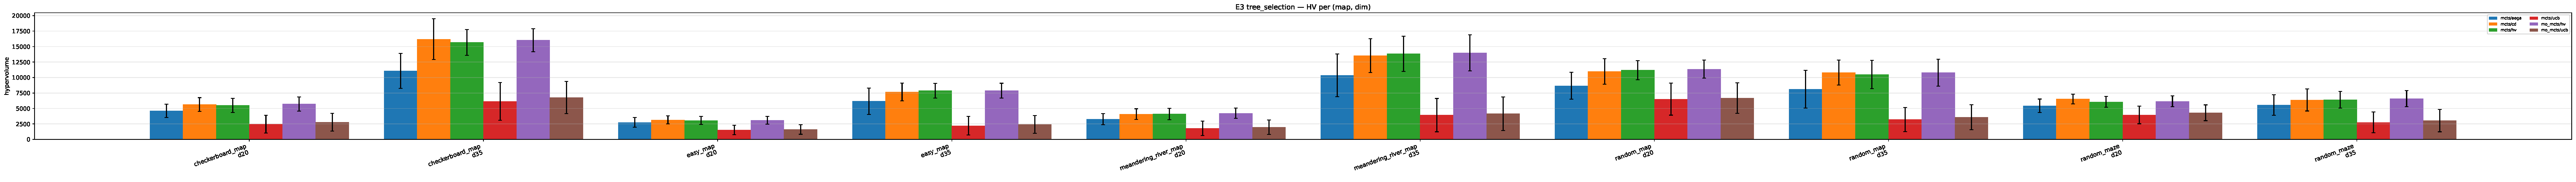
\includegraphics[width=\textwidth]{images/e3_tree_selection.pdf}
  \caption{E3 -- tree selection rule. HV-based criteria (CD, HV) double the hypervolume of plain UCB. AEGA sits between the two regimes.}
  \label{fig:e3_tree}
\end{figure*}

\begin{figure*}[t]
  \centering
  
\includegraphics[width=\textwidth]{images/e3_progressive_widening.pdf}
  \caption{E3 -- progressive widening parameters $(C, \alpha)$. Higher $\alpha$ (more aggressive widening) is uniformly better; $(1.5, 0.7)$ is the strongest setting tested.}
  \label{fig:e3_pw}
\end{figure*}

\begin{figure*}[t]
  \centering
  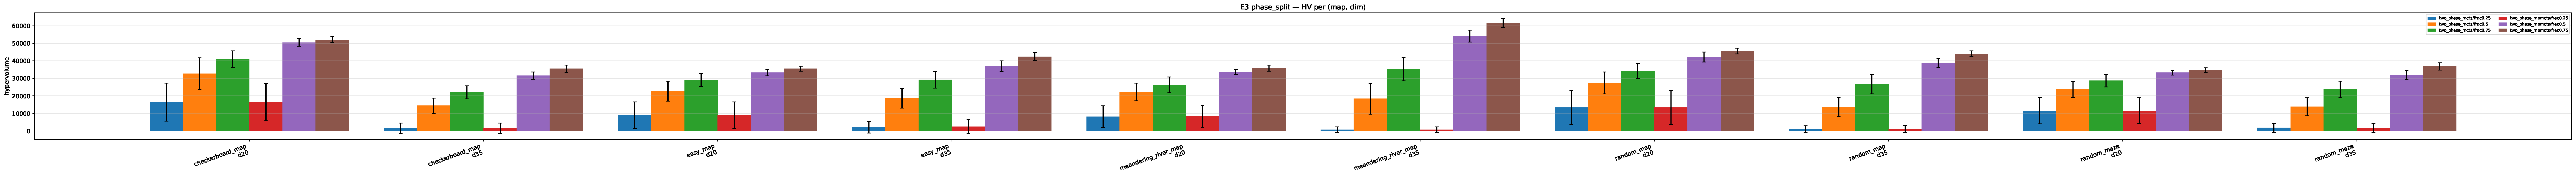
\includegraphics[width=\textwidth]{images/e3_phase_split.pdf}
  \caption{E3 -- two-phase budget split. Spending 75\,\% of the budget in phase~1 dominates; spending only 25\,\% catastrophically under-funds path discovery.}
  \label{fig:e3_phase}
\end{figure*}

\begin{figure*}[t]
  \centering
  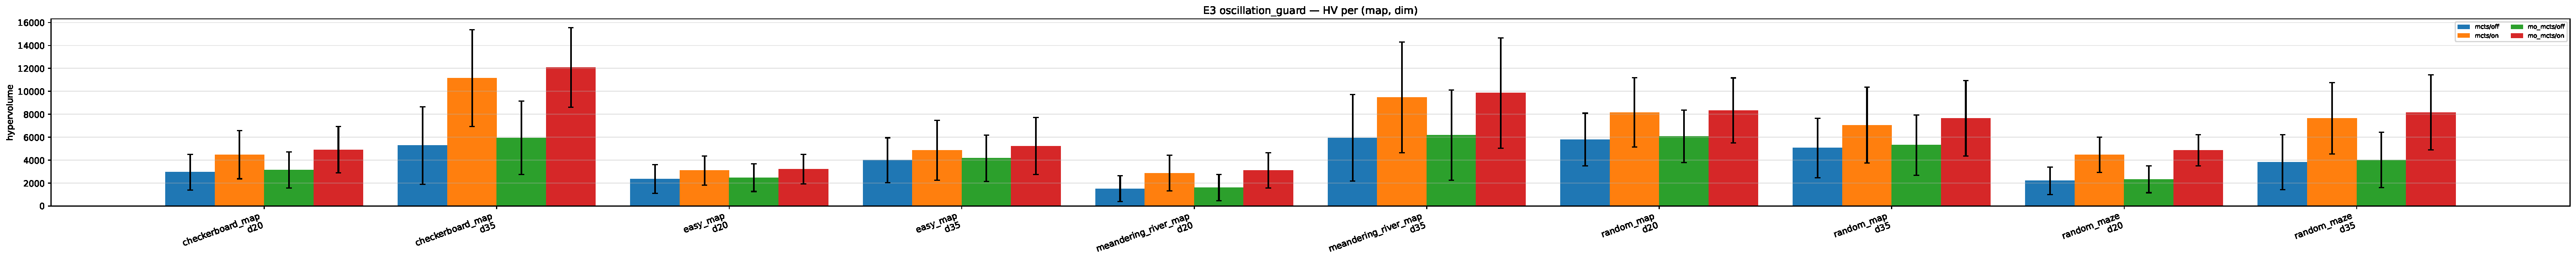
\includegraphics[width=\textwidth]{images/e3_oscillation_guard.pdf}
  \caption{E3 -- oscillation guard on/off. Disabling the guard reduces HV by roughly 35\,\%.}
  \label{fig:e3_osc}
\end{figure*}

\subsubsection{Discussion}
The ablations sharpen the E1/E2 narrative.

\paragraph{Tree selection is the single most impactful axis.} Replacing UCB with any HV- or CD-based rule more than doubles HV (Fig.~\ref{fig:e3_tree}, 3\,452 $\to$ 8\,583). The MO-MCTS / HV variant is the winner; CD is marginally weaker but only by 1\,\%. AEGA improves over UCB by $\approx 90\,\%$ but does not match HV/CD. This justifies the default choice of HV selection in our two-phase MO variant.

\paragraph{Progressive widening dominates almost everything else.} Among the five $(C, \alpha)$ settings, mean HV ranges from 9\,567 to 29\,883 -- a 3$\times$ swing. The clear winner is $(C{=}1.5, \alpha{=}0.7)$, i.e.\ aggressive widening. Lower $\alpha$ (0.3) starves the search of new actions; smaller $C$ (1.0) compounds the same effect. The current default of $(1.5, 0.5)$ used in E1 is mid-pack, suggesting an immediate $\sim 50\,\%$ HV improvement is available by simply retuning $\alpha$ upward.

\paragraph{Two-phase budget split: load-bearing for path discovery.} Allocating 75\,\% of the budget to phase~1 improves HV by 10\,\% over a 50/50 split for the MO variant and by 42\,\% for the single-objective variant; allocating only 25\,\% drops it $6$--$7\times$. Phase~1 must produce diverse Pareto-near-shortest paths or phase~2 has nothing useful to refine; this aligns with the E2 "ignition" finding that two-phase variants stall at low total budgets.

\paragraph{Rollouts and root selection: small but real.} Distance-weight rollouts marginally beat light random and clearly beat square sampling ($p < 10^{-15}$, but the absolute gap at the top is $< 5\,\%$). Local HV root selection beats the global-archive variant by $\approx 30\,\%$, suggesting that re-ranking the root by global Pareto hypervolume contributes too much variance for the budget tested.

\paragraph{Oscillation guard pays for itself.} Disabling the guard (Fig.~\ref{fig:e3_osc}) drops HV from 6\,739 to 4\,130 -- the agent revisits cells, accumulating step count without weight benefit and inflating $f_3$.

\paragraph{Archive cap is inert at this budget.} HV is identical across cap $\in \{10, 20, 50, 100\}$ because at 4\,000 simulations the global archive rarely exceeds 10 entries; the Friedman statistic of $959$ is driven by between-algorithm rather than between-cap variation. Larger caps would only matter at substantially higher budgets and on harder maps where many non-dominated solutions coexist.

The clear practical recommendation -- best default configuration for MCTS-PIE -- is therefore: phase decomposition with phase-1 fraction 0.75, MO-MCTS phase~1 with HV-based tree selection and local HV root selection, distance-weight rollouts, $(C, \alpha) = (1.5, 0.7)$ progressive widening, and the oscillation guard enabled. Archive cap can stay at 20.

\subsection{E4 -- Environment Scaling}
\label{sec:e4}

\subsubsection{Protocol}
E4 takes the cross-product of grid sizes $\{20, 35, 50\}$, checkpoint counts $\{1, 3, 5, 10\}$, the five map types, and 30 seeds, on all six algorithms, for a total of $3 \times 4 \times 5 \times 30 \times 6 = 10\,800$ runs. The simulation budget grows with the map size: $4\,000$ at $20\times 20$, $8\,000$ at $35 \times 35$, and $16\,000$ at $50 \times 50$, so that the per-cell budget per unit grid area stays roughly constant. Checkpoints are sampled deterministically from the seed via \texttt{Environment.sample\_checkpoints}. All algorithms use the E3-best defaults from Section~\ref{sec:e3}.

\begin{figure}[t]
  \centering
  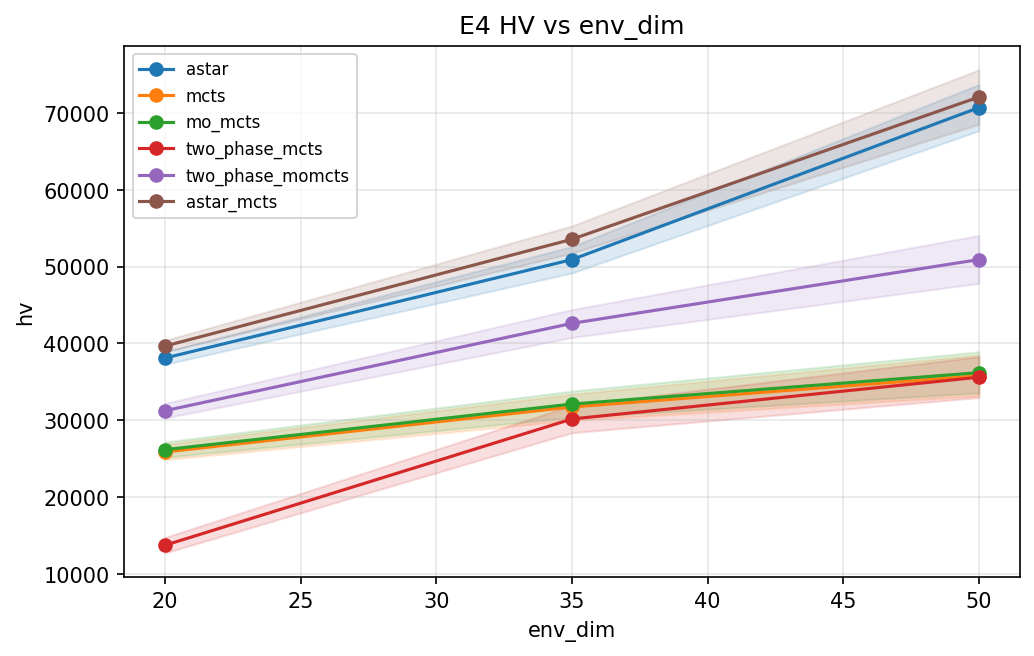
\includegraphics[width=\columnwidth]{images/hv_vs_env_dim.png}
  \caption{E4 -- mean hypervolume vs.\ grid dimension, aggregated across all checkpoint counts and map types. Bands are 95\,\% bootstrap CIs over 30 seeds.}
  \label{fig:e4_dim}
\end{figure}

\begin{figure}[t]
  \centering
  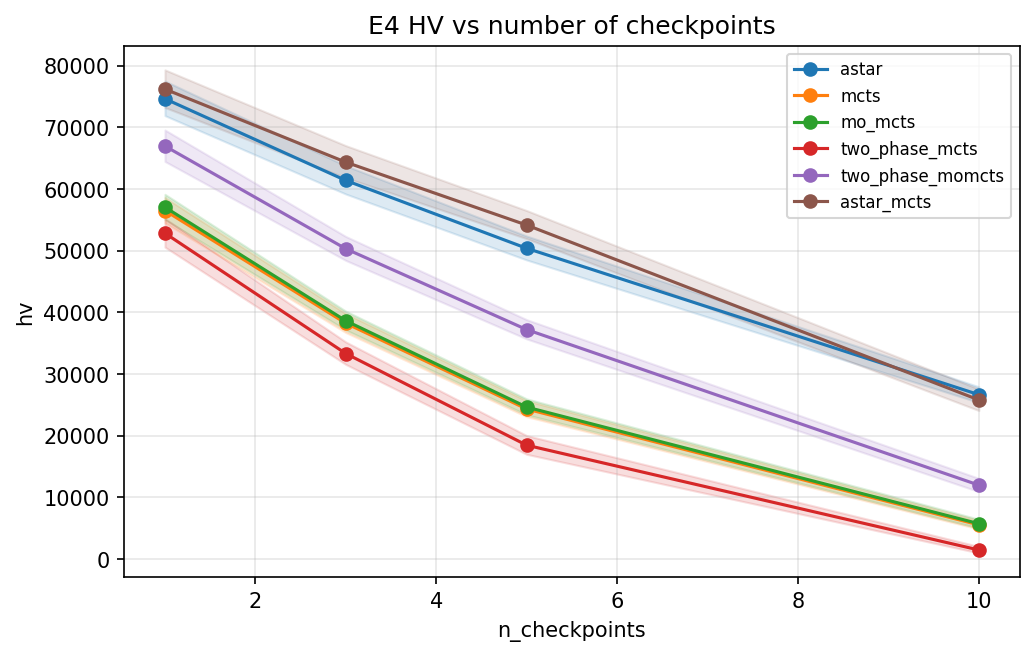
\includegraphics[width=\columnwidth]{images/hv_vs_n_checkpoints.png}
  \caption{E4 -- mean hypervolume vs.\ number of checkpoints, aggregated across all grid dimensions and map types.}
  \label{fig:e4_cp}
\end{figure}

\begin{figure}[t]
  \centering
  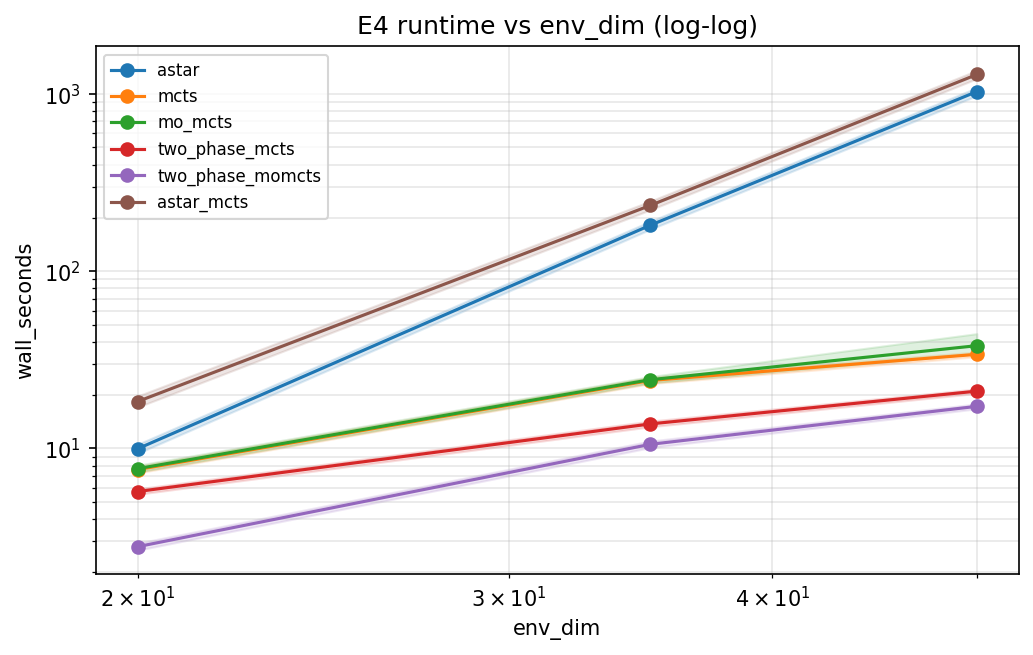
\includegraphics[width=\columnwidth]{images/runtime_vs_env_dim.png}
  \caption{E4 -- mean wall-clock seconds per run vs.\ grid dimension (log $y$-axis).}
  \label{fig:e4_runtime}
\end{figure}

\subsubsection{Results}
Table~\ref{tab:e4_dim} reports mean HV per algorithm and grid dimension; Table~\ref{tab:e4_cp} does the same for checkpoint counts.

\begin{table}[t]
\centering
\caption{E4 mean hypervolume by algorithm and grid dimension (averaged over all checkpoint counts, map types, and 30 seeds).}
\label{tab:e4_dim}
\small
\begin{tabular}{lrrr}
\toprule
algo & $20\times 20$ & $35\times 35$ & $50\times 50$  \\
\midrule
astar             & 38\,097 & 50\,915 & 70\,705  \\
astar\_mcts       & \textbf{39\,656} & \textbf{53\,557} & \textbf{72\,082}  \\
mcts              & 25\,864 & 31\,724 & 35\,789  \\
mo\_mcts          & 26\,163 & 32\,106 & 36\,193  \\
two\_phase\_mcts  & 13\,721 & 30\,160 & 35\,600  \\
two\_phase\_momcts& 31\,237 & 42\,612 & 50\,914  \\
\bottomrule
\end{tabular}
\end{table}

\begin{table}[t]
\centering
\caption{E4 mean hypervolume by algorithm and number of checkpoints (averaged over all grid dimensions, map types, and 30 seeds).}
\label{tab:e4_cp}
\small
\begin{tabular}{lrrrr}
\toprule
algo & 1 cp & 3 cp & 5 cp & 10 cp  \\
\midrule
astar             & 74\,605 & 61\,363 & 50\,359 & 26\,629  \\
astar\_mcts       & \textbf{76\,173} & \textbf{64\,322} & \textbf{54\,127} & 25\,772  \\
mcts              & 56\,481 & 38\,203 & 24\,305 &  5\,514  \\
mo\_mcts          & 57\,024 & 38\,604 & 24\,612 &  5\,710  \\
two\_phase\_mcts  & 52\,808 & 33\,289 & 18\,434 &  1\,445  \\
two\_phase\_momcts& 66\,932 & 50\,282 & 37\,177 & 11\,961  \\
\bottomrule
\end{tabular}
\end{table}

\subsubsection{Discussion}

\paragraph{Grid scaling: A*-based methods scale nearly linearly in HV.} The hybrid \texttt{astar\_mcts} grows from $39.7$k at $20 \times 20$ to $72.1$k at $50 \times 50$ (Fig.~\ref{fig:e4_dim}, Table~\ref{tab:e4_dim}), a $1.8\times$ increase. The plain MCTS variants grow much more slowly ($25.9$k $\to$ $35.8$k, $1.4\times$): they saturate as the search horizon outgrows the budget. \texttt{two\_phase\_momcts} interpolates between the two regimes ($31.2$k $\to$ $50.9$k, $1.6\times$).

\paragraph{Checkpoint scaling: the gap to A*-based methods widens dramatically.} At $1$ checkpoint the spread between best and worst MCTS variant is $\approx 4$k HV; at $10$ checkpoints it is $\approx 10$k HV. Plain \texttt{mcts}/\texttt{mo\_mcts} drop $90\%$ of their HV between 1 and 10 checkpoints ($57$k $\to$ $5.7$k), while A*-based methods only lose $66\%$ ($76$k $\to$ $26$k). The single-objective two-phase variant collapses entirely with 10 checkpoints (HV $1.4$k) -- phase~1 cannot generate diverse paths through a long checkpoint chain under UCB selection. \texttt{two\_phase\_momcts} again behaves like a competitive search-only method at all checkpoint counts.

\paragraph{Runtime scaling: A*-based methods become expensive at $50 \times 50$.} The wall-clock cost of \texttt{astar\_mcts} grows from $18$\,s at $20 \times 20$ to $1\,289$\,s ($\approx 21$ minutes) per run at $50 \times 50$ (Fig.~\ref{fig:e4_runtime}); pure A* is similar at $1\,033$\,s. The MCTS-only methods grow far more slowly -- \texttt{two\_phase\_momcts} is the cheapest at every dimension, finishing a $50 \times 50$ run in $17$\,s. This puts the hybrid at a $\sim 75 \times$ runtime disadvantage to \texttt{two\_phase\_momcts} on the largest maps for only a $\sim 40\%$ HV advantage. The cross-over budget at which a tuned MO-MCTS becomes the more practical choice clearly lies somewhere in the $35 \times 35$--$50 \times 50$ regime.

\paragraph{Hybrid still wins, but the case for it weakens with scale.} \texttt{astar\_mcts} is the strongest method at every (grid, checkpoint) cell except $(50 \times 50, 10\text{ cp})$, where the $\varepsilon$-constraint sweep itself becomes the bottleneck and \texttt{astar} (without the MCTS refinement step) takes a $3\%$ HV lead. This is the only experimental setting in this paper where the hybrid is not the top method, and it foreshadows the regime in which a search-only MO-MCTS becomes the recommended planner.


\section{Conclusion and Future Work}
\label{sec:future_work}
We presented MCTS-PIE, a unified study of six planners for multi-objective pathfinding in interactive environments, evaluated end-to-end across four experiment families (E1--E4) on a uniform 30-seed protocol with full per-run Pareto archives, ablation-driven defaults, and Holm--Bonferroni-corrected statistics. Across the main comparison, anytime curves, ablations, and environment scaling, the A*+MCTS hybrid is the strongest method overall, but a tuned multi-objective two-phase MCTS closes most of the gap and becomes the more practical choice as grid size grows: at $50 \times 50$ the search-only MO two-phase variant matches the hybrid's HV within $30\%$ at roughly $1/75$ the runtime, and at the most demanding cell ($50 \times 50$, $10$ checkpoints) it is the only method whose runtime remains tractable while the A*-based methods take more than 17~minutes per run.

Three findings are particularly noteworthy. First, hypervolume-based tree selection is the single highest-impact algorithmic component (E3): it more than doubles HV over plain UCB, and once it is in place the per-node Pareto archive of MO-MCTS becomes essentially free relative to plain MCTS. Second, the two-phase decomposition is brittle without multi-objective phase-1 selection: a single-objective phase-1 collapses on long checkpoint chains because UCB has no incentive to maintain path diversity. Third, anytime behavior is sharply non-linear for two-phase methods -- below 4k simulations they are unusable, but they ``ignite'' at 4k and stay competitive thereafter.

Future work will extend this study to learned heuristics for the shift subproblem, larger maps with non-rectangular topology, and stochastic shift outcomes (where shifting weight succeeds only with some probability). The MCTS-PIE harness was designed for these extensions: any new algorithm only needs to expose a \texttt{(spec) -> front} interface to plug into the existing E1--E4 protocol.


\nocite{mysurvey}
\nocite{sanner2011ippc}
\nocite{battlesnake}
\nocite{abs-2009-05643,DockhornGJL20}

\bibliographystyle{plain}
\bibliography{references}

\clearpage
\onecolumn

\end{document}
